\documentclass[letterpaper,10pt]{article}

%\setlength{\parindent}{0in}
%\usepackage{fullpage} 
\usepackage{amsmath}
\usepackage{amssymb}
\usepackage{enumerate}
\usepackage{graphicx}
\usepackage[table]{xcolor}
\usepackage{dcolumn}
\oddsidemargin 0.0in
\textwidth 6.5in
\newcolumntype{.}{D{.}{.}{-1}}
\newcommand*{\myalign}[2]{\multicolumn{1}{#1}{#2}}

%opening
\title{Final Exam}
\author{Steve Mazza}
%\date{December 9, 2011}

\begin{document}
\maketitle

\begin{description}
\item[Question 1:]
Given the differential equation $\dfrac{d^4y}{dx^4}+\dfrac{d^2y}{dx^2}=0\equiv y''''+Ay''$ derive the equivalent system of first-order ordinary differential equations.  This is a fourth order differential equation.  What order is the system of equations?  Is the system linear or nonlinear?  What does such a system of first-order ordinary differential equations represent?

% On problem 1 try treating the x derivatives like time derivatives.  That is, change x to t, and see if that makes it any clearer what to do.  When you have an answer change t back to x.  I believe this kind of problem is treated in either chapter 1 or 2 of Strogatz.

Change the variables as follows:
\begin{align*}
  y_1 &= y'' \\
  y_2 &= y'''' \\
  y_1'' &= y_2 \\
  y_2'' &= y_2 + Ay_1
\end{align*}
The system is second order since there are two variables.  This system is linear since all of the $y$-values on the right hand side of the equations are first order.  This looks a little like the equation for a dampened harmonic oscillator.

\item[Question 2:]
The Maxwell-Bloch equations are a sophisticated model for a laser and describe the dynamics of the electric field $E$, the mean polarization of the atoms $P$, and the population inversion $D$:
\begin{align*}
\dot{E} &= (P-E) \\
\dot{P} &= \gamma_1(ED-P) \\
\dot{D} &= \gamma_2(\lambda+1-D-EP)
\end{align*}
where $\gamma_1$ and $\gamma_2$ are decay rates of the atomic polarization and population inversion, respectively, and $\lambda$ is a pumping energy parameter.  The parameter $\lambda$ may be positive, negative, or zero; all other parameters are positive.  In the simplest case, $P$ and $D$ relax rapidly to steady values, and hence may be eliminated as follows.
\begin{enumerate}
\item Assuming $\dot{D}\approx 0$\ $\dot{P}\approx 0$, express $P$ and $D$ in terms of $E$, and thereby derive a first-order equation for the evolution of $E$.
\begin{align*}
	\gamma_1(ED-P)\approx0 &\implies ED-P\approx0 \\
	\gamma_2(\lambda+1-D-EP)\approx0 &\implies \lambda+1-D-EP\approx0 \\
	\mbox{So,\ } P\approx E\left(\frac{1+\lambda}{E^2+1}\right) &\mbox{and\ } D\approx\frac{1+\lambda}{E^2+1} \\
	\mbox{Applying\ } \dot{E} &= P-E \\ 
	\mbox{We obtain\ } \frac{dE}{dt} &= E\left(\frac{\lambda-E^2}{E^2+1}\right)
\end{align*}
\item Find all the fixed points of $E$.  \\ These occur at $\pm\sqrt{\lambda}\ \forall\ \lambda\geq0$ and $E=0$.
\item Draw the bifurcation diagram of $E^*$ versus $\lambda$.  Distinguish between stable and unstable branches. \\
  I'm not completely convinced I've gotten this code right and so the resulting plot may also be slightly incorrect, but it should not be too far off.  The graphic was generated in Mathematica.
  \begin{verbatim}
f[x_][a_] := a*((x - a^2)/(a^2 + 1));

cps[a_] =  x /. Quiet[Solve[D[f[a][x], x] == 0, x], 
   Solve::ratnz]

criticalOrbits[a_, cp_] := Module[{try},
   If[Head[cp] === Real,
    try = NestWhileList[f[a], cp, Abs[#] < 100 &, 1, 500];
    If[Abs[Last[try]] >= 100, try = {},
     try = Drop[{a, #} & /@ try, 100]
     ], {}]];
points[k_] := Partition[Flatten[Table[criticalOrbits[a, cps[a][[k]]],
    {a, -2, 4, 0.002}]], 2]

Graphics[{Opacity[0.02], PointSize[0.002],
  Table[{ColorData[1, l], Point[points[l]]},
   {l, 1, Length[cps[a]]}]}, Axes -> True, 
 AxesLabel -> {\[Lambda], \[CapitalEpsilon]}, 
 LabelStyle -> Directive[Blue, Bold]
  \end{verbatim}
  \begin{center}
    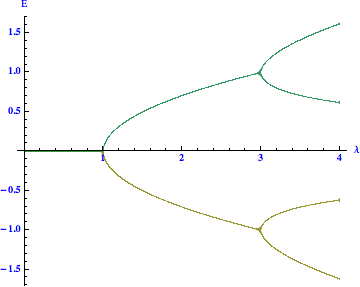
\includegraphics[scale=0.75]{images/problem2.png}
  \end{center}
  Stable regions should be near the zero at E.  The area beyond the first bifurcation between the $\lambda$-axis and the graph lines is unstable.
\end{enumerate}

\item[Question 3:]
What is this an example of?  What features are represented?
\begin{center}
  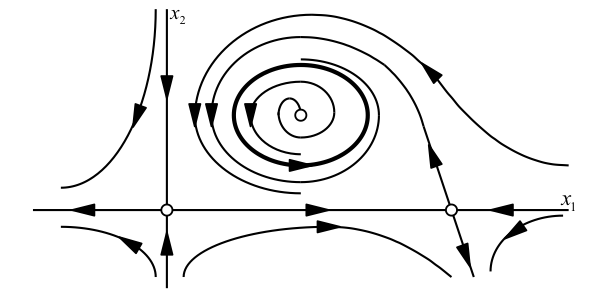
\includegraphics[scale=0.65]{images/phaseportrait.png}
\end{center}

This is a phase portrait.

From our class notes where this image was taken, ``A phase portrait is a qualitative picture of the behavior of a system in phase space.  Typically it shows fixed points, the stability of fixed points, closed orbits, and trajectories near the fixed points and closed orbits.  The phase portrait above is illustrative only and does not represent a specific system.''

Fixed points on this diagram are represented by the hollow dots. There are three; one appears at the intersection of the axes, one appears at the zero on the $x-$axis, and the third is located at the center of the sync of the closed orbit.  The closed orbit, located near the center of the diagram, is represented by the heavier closed line with the counter-clockwise directional arrow.

There are trajectories located near the fixed points which indicate stability or instability.  Trajectories moving toward fixed points indicate stability.  Trajectories moving away from fixed points indicate instability.  As seen in our diagram, a fixed point may be stable in one direction and instable in another.  A geometric representation of this would be a saddle point.  The unstable fixed point inside the closed orbit could be geometrically represented as a hill of bump in the
landcape.

\item[Question 4:]
For the Lorenz equations
\begin{align*}
\dot{x} &= \sigma(y-x) \\
\dot{y} &= rx-y-xz \\
\dot{z} &= xy-bz
\end{align*}
with $\sigma=10, r=28$, and $b=2.66666$, and initial condition $x=1.0+\delta, y=1.0$, and $z=10$, determine how long it takes the absolute error between the ``true $x$ solution'' $(\delta=0)$ to grow from $\delta$ to 0.1. Calculate for $\delta$ values of 0.01, $10^{-4}, 10^{-6}, 10^{-8}$, and $10^{-10}$.  What does this tell you about the predictability versus measurement error?  Can you estimate the Liapunov exponent?

% On problem 4, the solution using the initial conditions gives you the “true” result.  When those initial conditions are varied by adding 0.01, 0.0001, etc., the difference between the resulting solution and the true solution is the error.  Absolute error is the absolute value of the error.

Solution with unaltered initial conditions.
\begin{verbatim}
NDSolve[{x'[t] == 10*(y[t] - x[t]), 
   y'[t] == -x[t] z[t] + 28* x[t] - y[t], 
   z'[t] == x[t] y[t] - (8/3)*z[t], x[0] == 1.0, z[0] == 10, 
   y[0] == 1.0}, {x, y, z}, {t, 0, 200}, MaxSteps -> Infinity];
\end{verbatim}
\begin{center}
  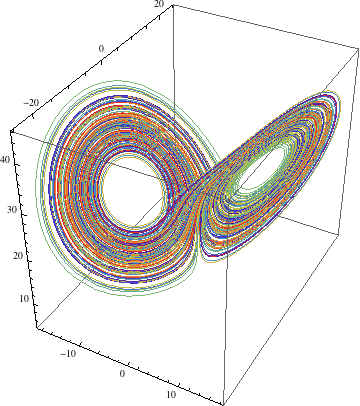
\includegraphics[scale=0.5]{images/lorenz0.png}
\end{center}
Iterated with $\delta=0.1$, the map looks considerably different.
\begin{center}
  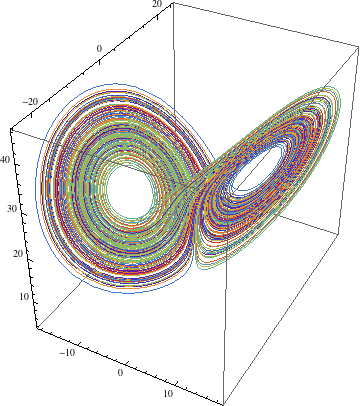
\includegraphics[scale=0.5]{images/lorenz1.png}
\end{center}
Iterated with $\delta=0.01$.
\begin{center}
  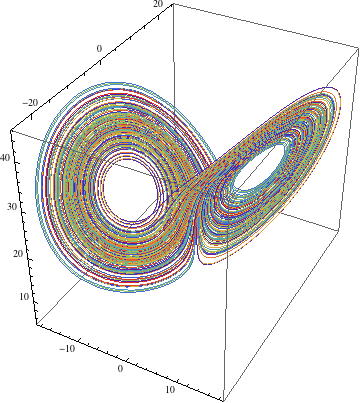
\includegraphics[scale=0.5]{images/lorenz2.png}
\end{center}
Iterated with $\delta=10^{-4}$.
\begin{center}
  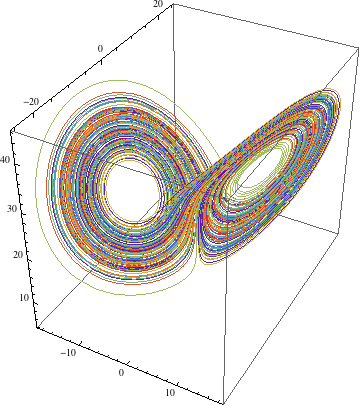
\includegraphics[scale=0.5]{images/lorenz3.png}
\end{center}
Iterated with $\delta=10^{-6}$.
\begin{center}
  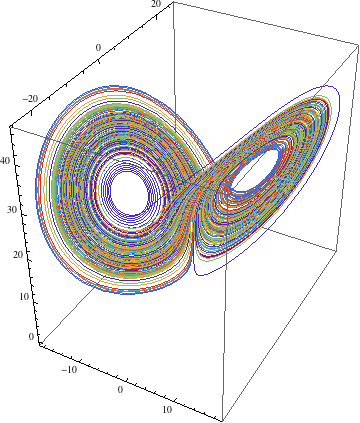
\includegraphics[scale=0.5]{images/lorenz4.png}
\end{center}
Iterated with $\delta=10^{-8}$.
\begin{center}
  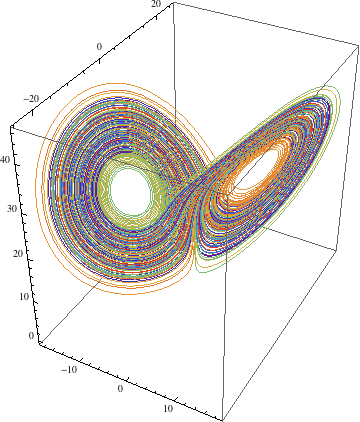
\includegraphics[scale=0.5]{images/lorenz5.png}
\end{center}
Iterated with $\delta=10^{-10}$.
\begin{center}
  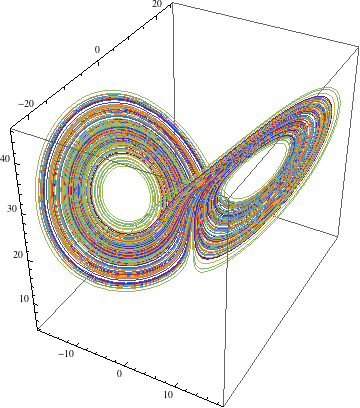
\includegraphics[scale=0.5]{images/lorenz6.png}
\end{center}
This seems to indicate that measurement error greatly affects predictability.

\item[Question 5:]
Consider the iterated map given by
\[x_{n+1} = \left\{
  \begin{array}{lr}
    rx_n &  0\le x_n \le 0.5 \\
    r(1-x_n) &  0.5\le x_n \le 1
  \end{array}
\right.
\]
where $0<r<2$.  What properties do you expect to see in the orbit diagram?  Is there any condition that might cause different behavior?  The Liapunov exponent is $\lambda=\mbox{ln\ }r$. What does this tell you about the behavior?

% On problem 5 think about the similarity of the tent map to the logistics map.  The orbit diagram is the plot of the allowed values of the function as a function of the parameter r.

This is (obviously) a piecewise function and so its behavior is highly dependent on the values of $x$.  Inasmuch, it behaves similarly to the tent map.  Because the Liapunov exponent is positive, it suggests that there are chaotic solutions for $r>1$.

\item[Question 6:]
  In your own words and using no more than one paragraph, describe the difference between complex and complicated systems.  That is, in your own opinion what distinguishes the two?

  The difference between complexity and complicated systems hinges on the interactions of the parts of the system and on how difficult those interactions make predicting the future state of the system.  Emergent properties, a hallmark of complex systems, come from these highly affective interactions.  Note that systems with many moving parts and even possibly many interactions but whose outcomes are highly deterministic are not complex, but complicated.  The classic example of
  this is a watch.  Lastly, complex systems exhibit a robustness that merely complicated systems do not have.  That is, they will continue to function despite the loss of a (small) subset of its parts.

\item[Question 7:]
How are fractals and complexity related?

According to Mitchell (page 103, ``Complexity as Fractal Dimension''), the fractal dimension of an object is a measure of its complexity.  A fractal dimension is often a ratio (non-integer) that is a statistical index of complexity indicating how detail changes with scale.  This is also referred to as the Hausdorf dimension and quantifies the number of self-similar copies at each level of magnification.

\item[Question 8:]
Define what an adaptive agent-based model is and briefly describe its characteristics.

Agent-based models are network computer models  were the agents play a central role in the modeling. They facilitate the exploration of complex systems in great detail.  Agents of various types (of classes) may have different properties regarding memory, movement, and cognitive ability.  Behaviors of agents are interdependent.

While there may be several (or many) classes of agents, they all behave based on a set of rules which may be either fixed (as in Conway's Game of Life) or adaptive.  Either way, the agents themselves drive the evolution of the model through actions (or non-action) and interactions.  Actions might look spacial as in changing location or may be logical as in changing a strategy (e.g., from cooperation to defection).

The rules in an agent-based model are often threshold-based.  When a critical level is reached (high or low), a rule is triggered.  This may have either positive or negative feedback, encouraging either more or less of the same action.

In the case of adaptive agents, the rules are not fixed.  Rather the agents follow meta-rules that determine the ways in which the current rule set may be altered.  Especially under these conditions, but also true in general, agent-based systems often exhibit complex and emergent behavior.

\item[Question 9:]
In an engineering system consisting of various parts and mechanisms, what kinds of diversity are most applicable to determining complexity?  How might that diversity be measured?

There are three rules of thumb that inform our understanding of diversity with respect to how it determines complexity.
\begin{itemize}
  \item Variation within a type seldom results in complexity.
  \item Differences between types is often associated with complexity.
  \item Diversity in composition is often associated with complexity.
\end{itemize}

In addition, there are four types of problems where exploration (increased diversity) is particularly useful.
\begin{enumerate}
  \item Long-term or widespread problems.  Assuming there is an investment cost in encouraging diversity, the longer you have to amortize the cost of finding a solution, the greater the payoff.
  \item Problems that provide fast, reliable feedback.  These are almost always worth pursuing and are often characterized as low hanging fruit.  Improvements tend to happen quickly under conditions of rapid and reliable feedback.  And the early win afforded such a solution provides more time for the solution to work.
  \item Problems that are unlikely to result in catastrophe.  This establishes the premise for basing exploration (encouraging diversity) on a risk for reward basis.  If the risk of extending diversity is low then we may be more willing to pursue this strategy.
  \item Problems that have looming disasters. When in a situation where the status quo will eventually lead to a disastrous end then the risk of encouraging diversity should be weighed against the risk of \emph{not} encouraging diversity.
\end{enumerate}

\item[Question 10:]
What approaches are likely to [be] part of any attempt to harness complexity in an inherently complex system?

Traditional approaches to control (command and control) fail for complex systems.  Complex systems, however, can be harnessed by considering the primary characteristics of interdependence, connectedness, diversity, and adaptivity.  One way to harness complexity is to adjust diversity, which determines the level of exploitation or exploration.  Increasing diversity moves the system away from exploitation toward exploration.  To a point, increasing diversity helps prevent errors
(Linus' Law).

Watch for outliers in a population.  It does not take many vocal people to sway the conditions of a complex system.  Be wary of spending too much effort chasing small gains in efficiency and always leave room in the system so that failure does not cascade (as in recent bank failures).

Adjusting the interactions to remove unnecessary connections in favor of synergistic ones is another strategy.  Incentives may not support your desired outcomes.  In hierarchical structures, severing connections to parent organizations increases diversity and exploration.

Additionally, in ``Harnessing Complexity,'' Axelrod \& Cohen present a framework for harnessing complexity, which the refer to as the Complex Adaptive Systems approach.  They describe various techniques of variation, interaction, and selection that the user of a system can leverage to affect or sway the outcome of a complex adaptive system.

The following ideas are summarized from the section titled, ``What a User of the Framework Can Do,'' in the \emph{Conclusion} of their book.

\begin{description}
  \item[Variation] \ \\
    \begin{itemize}
      \item Arrange organizational routines to generate a good balance between exploration and exploitation.
      \item Link processes that generate extreme variation to processes that select with few mistakes in the attribution of credit.
    \end{itemize}
  \item[Interaction] \ \\
    \begin{itemize}
      \item Build networks of reciprocal interaction that foster trust and cooperation.
      \item Assess strategies in light of how their consequences can spread.
      \item Promote effective neighborhoods.
      \item Do not sow large failures when reaping small efficiencies.
    \end{itemize}
  \item[Selection] \ \\
    \begin{itemize}
      \item Use social activity to promote the growth and spread of valued criteria.
      \item Look for shorter-term, finer-grained measures of success that can usefully stand in for longer-run, broader goals.
    \end{itemize}
\end{description}

Detailed explanations of these approaches can be found on pages 155 -- 158.

\end{description}
\end{document}
